\chapter{Change detection - related work}  %Title of the First Chapter
%\ifpdf
%    \graphicspath{{D:/MyTemp/gitlocal/phd-thesis/text/chapter1/img/}}
%%\graphicspath{{chapter1/img/}{Chapter1/Figs/PDF/}{Chapter1/Figs/}}
%\else
%    \graphicspath{{Chapter1/Figs/Vector/}{Chapter1/Figs/}}
%\fi
%********************************** %First Section  **************************************

Def: Change point is a time moment $\tau$ dividing data stream of observations into subsets $B_j$ each of which can be regarded as a random sample from different an underlying probability distribution.

\section{CUSUM method}
In the CUSUM~\cite{Page1954} method the \cd happens by monitoring the output statistic calculated as an accumulated sum of the deviations from the mean level.



Figure~\ref{fig:cusum_demo1}
\begin{figure}
    \centering
        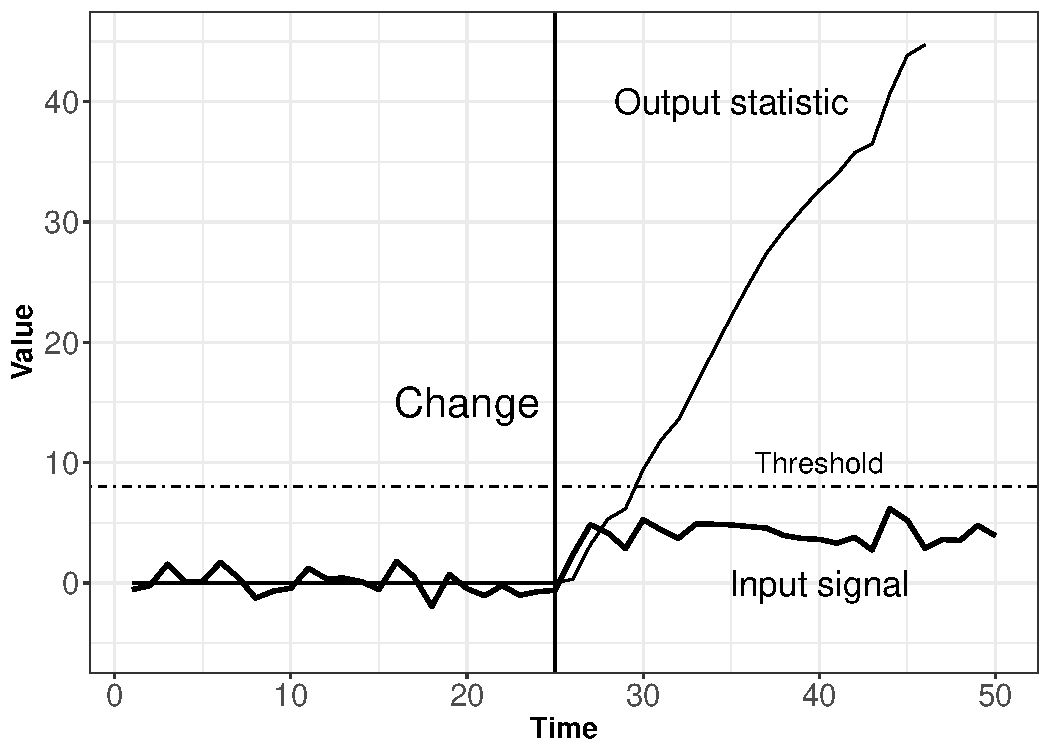
\includegraphics[width=0.8\textwidth]{./img/cusum_demo1.pdf}
    \caption{CUSUM example}
    \label{fig:cusum_demo1}
    % FIGURE source code: av-maslov.github.io/phd/plot2-cusum-demo:
\end{figure}

\subsection{Adaptive CUSUM}
From~\cite{luo2009adaptive}:``The standard cumulative sum chart
(CUSUM) is widely used for detecting small and moderate process
mean shifts, and its optimal detection ability for any
pre-specified mean shift has been demonstrated by its equivalence
to continuous sequential tests. In real practice, the assumption
of knowing the true mean shift in prior cannot be always met. So
it is desirable to design a procedure that is efficient for
detecting a range of future expected but unknown mean shifts.''

\section{ADWIN}
algorithm and example

Figure~\ref{fig:adwin_demo1}
\begin{figure}
    \centering
    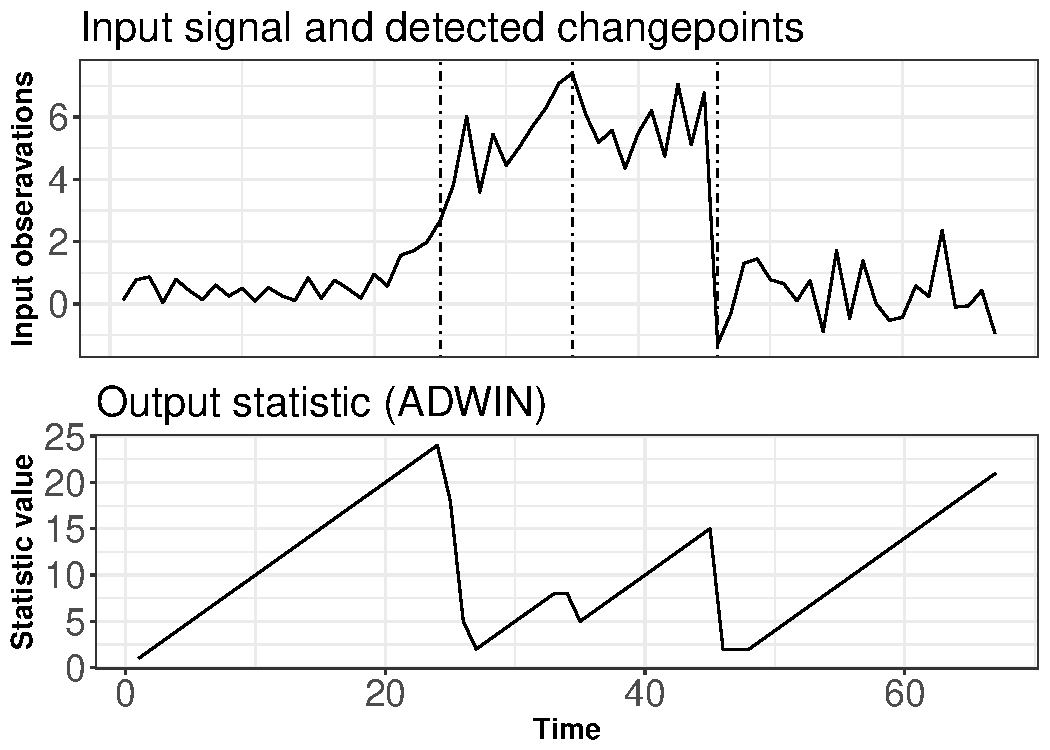
\includegraphics[width=0.8\textwidth]{./img/adwin_demo1.pdf}
    \caption{ADWIN example}
    \label{fig:adwin_demo1}
    % FIGURE source code: av-maslov.github.io/phd/plot2-cusum-demo:
\end{figure}

\section{Related work. State of the Art in On-line change detection}
% Off-line Changedetection settings -> Optimal
% location of the changepoints!
The optimality of the dynamic programming
algorithm for segme n is proved in
~\cite{Jackson2005}. It is proved there that the
proposed algorithm finds an optimal segmentation
given the cost function.

There are passive and active methods.  Active
methods determine whether and when a drift has
occurred before taking any actions.  Passive
update the online model continuously without an
explicit trigger reporting the drift.

\begin{itemize}
    
    \item Reviews~\cite{Polunchenko2011}
    ~\cite{WilsonBayesOnline},~\cite{TartakovskySeq}. Book~\cite{basseville1993detection}.
    
	\item Classical method is CUSUM~\cite{Page1954}
	
	\item In~\cite{mackay2007} authors propose a Bayesian approach for On-Line changedetection by applying an effective recursive message-passing algorithm to estimate a joint Pdf $P(r_t, x^{(1:t)})$ of run length latent variable $r_t$.
	
	\item ADWIN method is proposed in~\cite{bifet2007learning}. 
    BasicCounting problem~\cite{datar2002} and Exponential histogram (EH)-like data structure is used to speed up the basic ADWIN implementation.
	
	\item Early drift detection method (EDDM) proposed in~\cite{baena2006early}.
	
	\item Just-in-time adaptive classifiers are proposed in ~\cite{alippi2008just},~\cite{alippi2008just2},~\cite{AlippiRecConcept}
	
	\item MDL based detector~\cite{StreamKrimp}. KRIMP algorithm characterizes a probability distributions with code tables used by StreamKrimp to partition the stream into a sequence of substreams (???check).
    
    \item Bayesian approach
    % cited in paper by MacKay
    ~\cite{fearnhead2003line}.
    
    \item Concept drift: ~\cite{Widmer1996}
    
    \item A dynamic programming based algorithm BayesainBlocks to estimate optimal edges of the histogram proposed in~\cite{scargle2013studies}.
    
    \item Surfing wavelets~\cite{gilbert2001surfing}.
    
\end{itemize}



\subsection{Change detection example}
To illustrate how detectors work let's consider a widely used CUSUM detector~\cite{Page1954}.
CUSUM has two parameters: reference value $k$ related to the value of the desired change in the mean value to be detected and threshold $h$ for the output statistic $S$ calculated on-line and controlling sensitivity of the detector.
CDE is alarmed when $S > h$.
Output is shown in Figure~\ref{fig:detectorsbehaviour} where changes $\pmb{c}_{1:k}$ in the signal are depicted by vertical solid lines and CDEs $\pmb{c}_{1:l}^\ast$ are shown by dashed lines.
%Points considered by the detector as change points is a sequence of \textit{change detection events} (CDEs) (Figure~\ref{fig:detectorsbehaviour}).
%Subset of CDEs which correspond to actual changes in the signal are \textit{true positives} (TP).
%CDEs caused by outliers correspond to false alarms or \textit{false positives} (FP).
%Typical detector's output is depicted in Figure~\ref{fig:detectorsbehaviour},

The figure illustrates the effect of setting detector's sensitivity to higher~(left figure) and lower~(right figure) levels; with higher sensitivity all changes are detected, but there are also a lot of FPs, and with lower sensitivity there are no FPs, but changes are detected with a considerable delay.

\begin{figure*}
\centering
\begin{minipage}{0.45\textwidth}
%\includegraphics[height = 0.25\textheight, width=1.0\textwidth]{./images/Behv1.pdf}
%\includegraphics[width=1.0\textwidth]{./chapter1/images/Behv1.pdf}
\includegraphics[width=1.0\textwidth]{pics/changeDetection/Behv1.pdf}
\end{minipage}
\begin{minipage}{0.45\textwidth}
%\includegraphics[height = 0.25\textheight, width=1.0\textwidth]{./images/Behv2.pdf}
%\includegraphics[width=1.0\textwidth]{./chapter1/images/Behv2.pdf}
\includegraphics[width=1.0\textwidth]{pics/changeDetection/Behv2.pdf}
\end{minipage}
\caption{Univariate signal with 10 changes (depicted by vertical solid lines) in the mean value.
CDEs are shown by vertical dashed lines.
In case of higher sensitivity of the detector (left figure) all changes are detected with a small time delay but at the expense of a high number of FPs.
In case of lower sensitivity (right figure) there are fewer FPs, but the lag in change detection is big.}
\label{fig:detectorsbehaviour}
\end{figure*}


\section{Bayesian change detector}
~\cite{DowneyChp}
~\cite{MacKay_Inference_Book}
~\cite{gelman2013bayesian}
\subsection{Building blocks}
Conditional probability
\begin{equation} \label{eq:conditional_probability}
P(x|y) = \frac{P(x,y)}{P(y)}
\end{equation}
Marginal probability
\begin{equation}
P(x) = \int P(x,y) dy
\end{equation}
from the definition of conditional distribution we obtain a product rule
(chain rule)
\begin{equation}
P(x,y|H) = P(x|y,H) P(y|H) = P(y|x,H) p(x|H)
\end{equation}
rewriting marginal distribution we get sum rule
\begin{equation}
P(x|H) = \sum_y P(x,y|H) = \sum_y P(x|y,H)P(y|H)
\end{equation}
and Bayes theorem obtained from the product rule
\begin{equation}
P(y|x,H) = \frac{P(x|y,H) P(y|H)}{P(x|H)} = \frac{P(x|y,H) P(y|H)}{ \sum_{y'} P(x|y',H) P(y'|H) }
\end{equation}

Factorization of a joint distribution
\[
p(u,v,w) = p(u|v,w)p(v|w)p(w)
\]

\section{Bayesian \online change detection in a single time series}
%Important notes are in the iPython Notebook in "Changedetection.jl - python_code -"
Paper~\cite{mackay2007} describes the method for a constant value hazard rate $h$.
%\subsubsection{Integration with the Online Bayesian change detector}
The most natural way to integrate PCCF with the change detector is using Bayesian approach.
We illustrate this option using Bayesian \online \changepoint detection algorithm proposed in~\cite{mackay2007}.
Authors introduces a latent variable called run length $r_t$ which is the number of time steps since the last change point.
\Changepoint corresponds to the event when $r_t == 0$.
Prior distribution for the changes is given by the hazard rate $h$ which can be learnt \online~\cite{Wilson2010a}.
If we expect approximately one change per $100$ time steps then hazard rate is $h = 0.01$.
The drawback of this prior is that it is not-informative because it assigns equal change probabilities for every moment and does not allow to take into account possibility of the changes caused by outliers and noise.
% and on every time step we expect the change with probability $0.1$ and that .
%. specified as a set of conditions~\ref{eq:hazard_rate}
% and further extended in the work~\cite{Wilson2010a}.

We propose to use Gaussian PCCF as a prior in case of recurrent changes when additional information about average distance between changes is available in a form of parameters $(\mu, \sigma)$.
% in order to take into account additional information in a form of average distance between changes and skip possible noisy changes.
%In~\cite{mackay2007} authors used constant values hazard rate $h$  as a prior.
% PCCF is more informative prior in case of recurrent changes but it also has two parameters $(\mu, \sigma)$ instad of one $h$.

Detailed description of the \online Bayesian detector and pseudocode are available in the papers~\cite{mackay2007, Wilson2010a}.
Briefly, \online Bayesian change detector operates as follows.

\begin{equation}
p(r_t | r_{t-1}) =
\begin{cases}
1 - h \text{\:\:\: if }  r_t = r_{t-1} + 1 \\
h \text{\:\:\:\:\:\:\:\:\:\:\:  if } r_t = 0
\end{cases}
\label{eq:hazard_rate}
\end{equation}
$P(r_t, x_t) = P(r_t) P(x_t)$
\begin{multline}
P(r_2, x_1, x_2) = \sum_{r_1} P(r_2, r_1, x_2, x_1) = \\
\sum_{r_1} P(r_2, x_2 | r_1, x_1) P(r_1, x_1) = \\
\sum_{r_1} P(r_2 | r_1) P(x_2 | r_1, x_1) P(r_1, x_1)
\end{multline}
here $x^{1:r_1} == x_1$; $P(x2 | r1, x1)$ is defined by $r_1$ value. 
If $r_1 == 1$ then $P(x_2|...) = N(x_2|\mu=x_1, \sigma=...)$

Let's denote the most recent change as $c_{t-1}$. %vector of changes when $r_t == 0$
We propose
% Current moment of time is
\begin{equation}
p(r_t | r_{t-1}) =
\begin{cases}
\mathbb{P}(\tau -  t_s) \text{\:\:\: if }  r_t = r_{t-1} + 1 \\
\mathbb{P}(\tau -  t_s) \text{\:\:\:\:\:\:\:\:\:\:\:  if } r_t = 0
\end{cases}
\label{eq:hazard_rate_our}
\end{equation}

\section{\Online update of statistics}
Exponential family of distributions~\cite{murphy2007conjugate}
% Bishop 2.4, [p.113]
The exponential family of distributions over $\mvec{x}$, given parameters $\mvec{\eta}$, is a set of distributions of the form
\begin{equation}
p(\mvec{x} | \mvec{\eta}) = h(\mvec{x}) g(\mvec{\eta}) \exp\{\mvec{\eta}^T \mvec{u}(\mvec{x})\}
\label{eq:exponential_family}
\end{equation}
For the univariate Gaussian distribution $p(x|\mu,\sigma) = \GaussDistP$ the posterior for the mean value is~\cite{Blei} 
\begin{equation}
 E(\mu | x_{1:n}, \mu_0, \sigma_0^2) = \frac{\mu_0 / \sigma_0^2 + \sum_{i=1}{n} x_i }{1/\sigma_0^2 + n}
\end{equation} 
%and for the standard deviation 
%\begin{equation}
%
%\end{equation}

\subsection{CFB Data Description}
\label{sec:datasecription}
We have two datasets the first is CFB fuel mass
signal~\cite{ZliobaiteBP09}(Fig.~\ref{fig:CFBsig1}) 
\begin{figure}[htb!]
    \center
    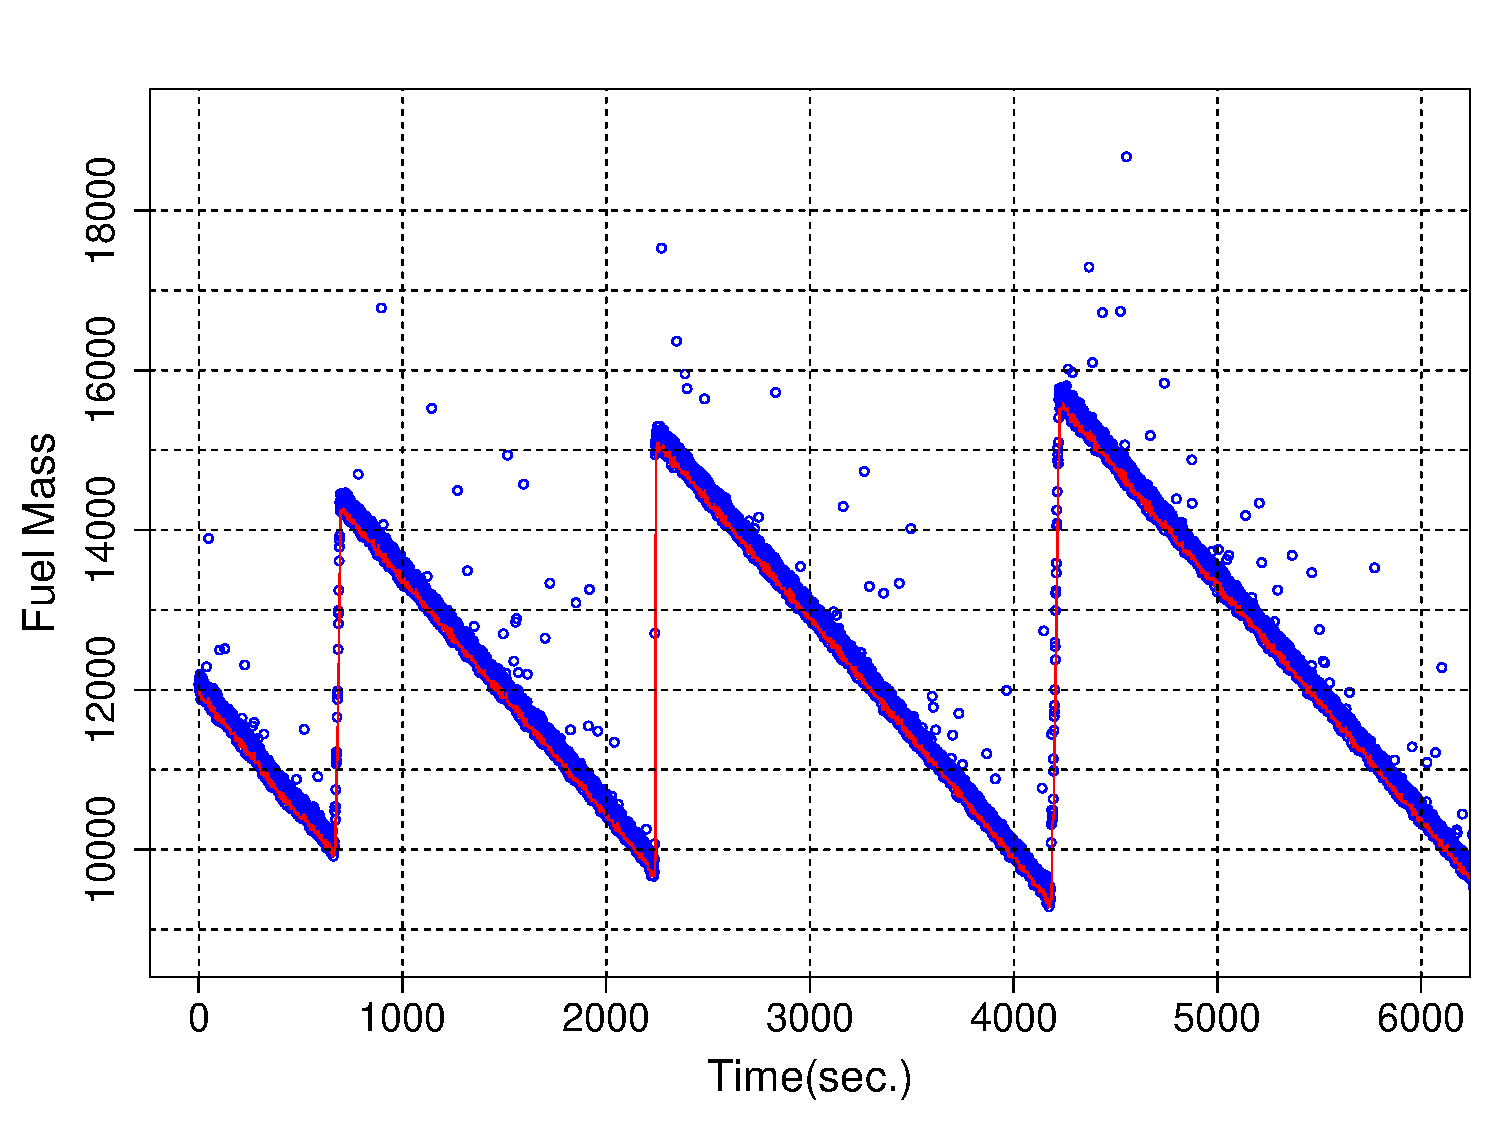
\includegraphics[width=0.45\textwidth]{pics/changeDetection/Part1DataA.pdf}
    \caption{CFB mass flow signal. There are burning(signal goes down) and
        feeding(signal goes up) regimes. Feeding regime is hard to detect because sometimes
        only one or two observations are being recorded.}
    \label{fig:CFBsig1}
\end{figure}


\subsection{Outliers detection}
%% \textit{Later this loess fitting will be replace by repaeted medians method.}\\
For outliers detection we use modified interquartile range test.
Firstly fitting curve is calculated to represent underlying
signal("ground truth").  After that scores on the basis of
interquartile range of residuals are assigned and outliers are
collected given threshold value for scores.

As a fitting curve we use loess(robust locally weighted) regression
curve ~\cite{Loess} which is not sensitive to outliers.  For each
$x_{i}$ in a moving window of length $n$, $q$ closest values are
selected ($q \leq n$) and each is given a weight $v_{i}$ based on it's
distance $\lambda_{q}(x)$ from $x_{i}$

\begin{equation}
v_{i}=W(\frac{|x_{i}-x|}{\lambda_{q}(x)})
\end{equation}

where $W$ is a tricube function $W(u)=(1-u^{3})^{3}$ for $0 \geq u < 1$
and equal to $0$ otherwise. Values $x$ close to $x_{i}$ have the largest weights.
After that weighted regression values of polynomial degree of $d$ are calculated.\\

Scores are calculated as follows.
Quartiles of set of values in a moving window are three points which
divide the data set into four equal groups.  First quartile $Q_{1}$
splits lowest $25\%$ od data, second quartile $Q_{2}$
(\textit{median}) divide data in a half and third $Q_{3}$ splits
highest $25\%$ of data.  Given quartiles $Q_{1},Q_{3}$ and
interquartile range $IQR=Q_{3}-Q_{1}$ score for for every point in a
moving window is calculated as follows.
Lower and upper limits are: $LL = Q_{1}-1.5*IQR$ and $UL = Q_{3}+1.5*IQR$.
On the Figure ~\ref{fig:OutliersExample} an example for sample from
normal distribution and one outlier is shown.
\begin{figure}[htb!]
\center
\includegraphics[width=0.55\textwidth]{pics/changeDetection/OutliersScore}
\caption{An example of time series with one outlier and corresponding
  calculated scores. Given the threshold value outliers are detected.}
\label{fig:OutliersExample}
\end{figure}
Results for real data are on the Figure ~\ref{fig:OutliersCFB4}.
\begin{figure}[htb!]
    \center
    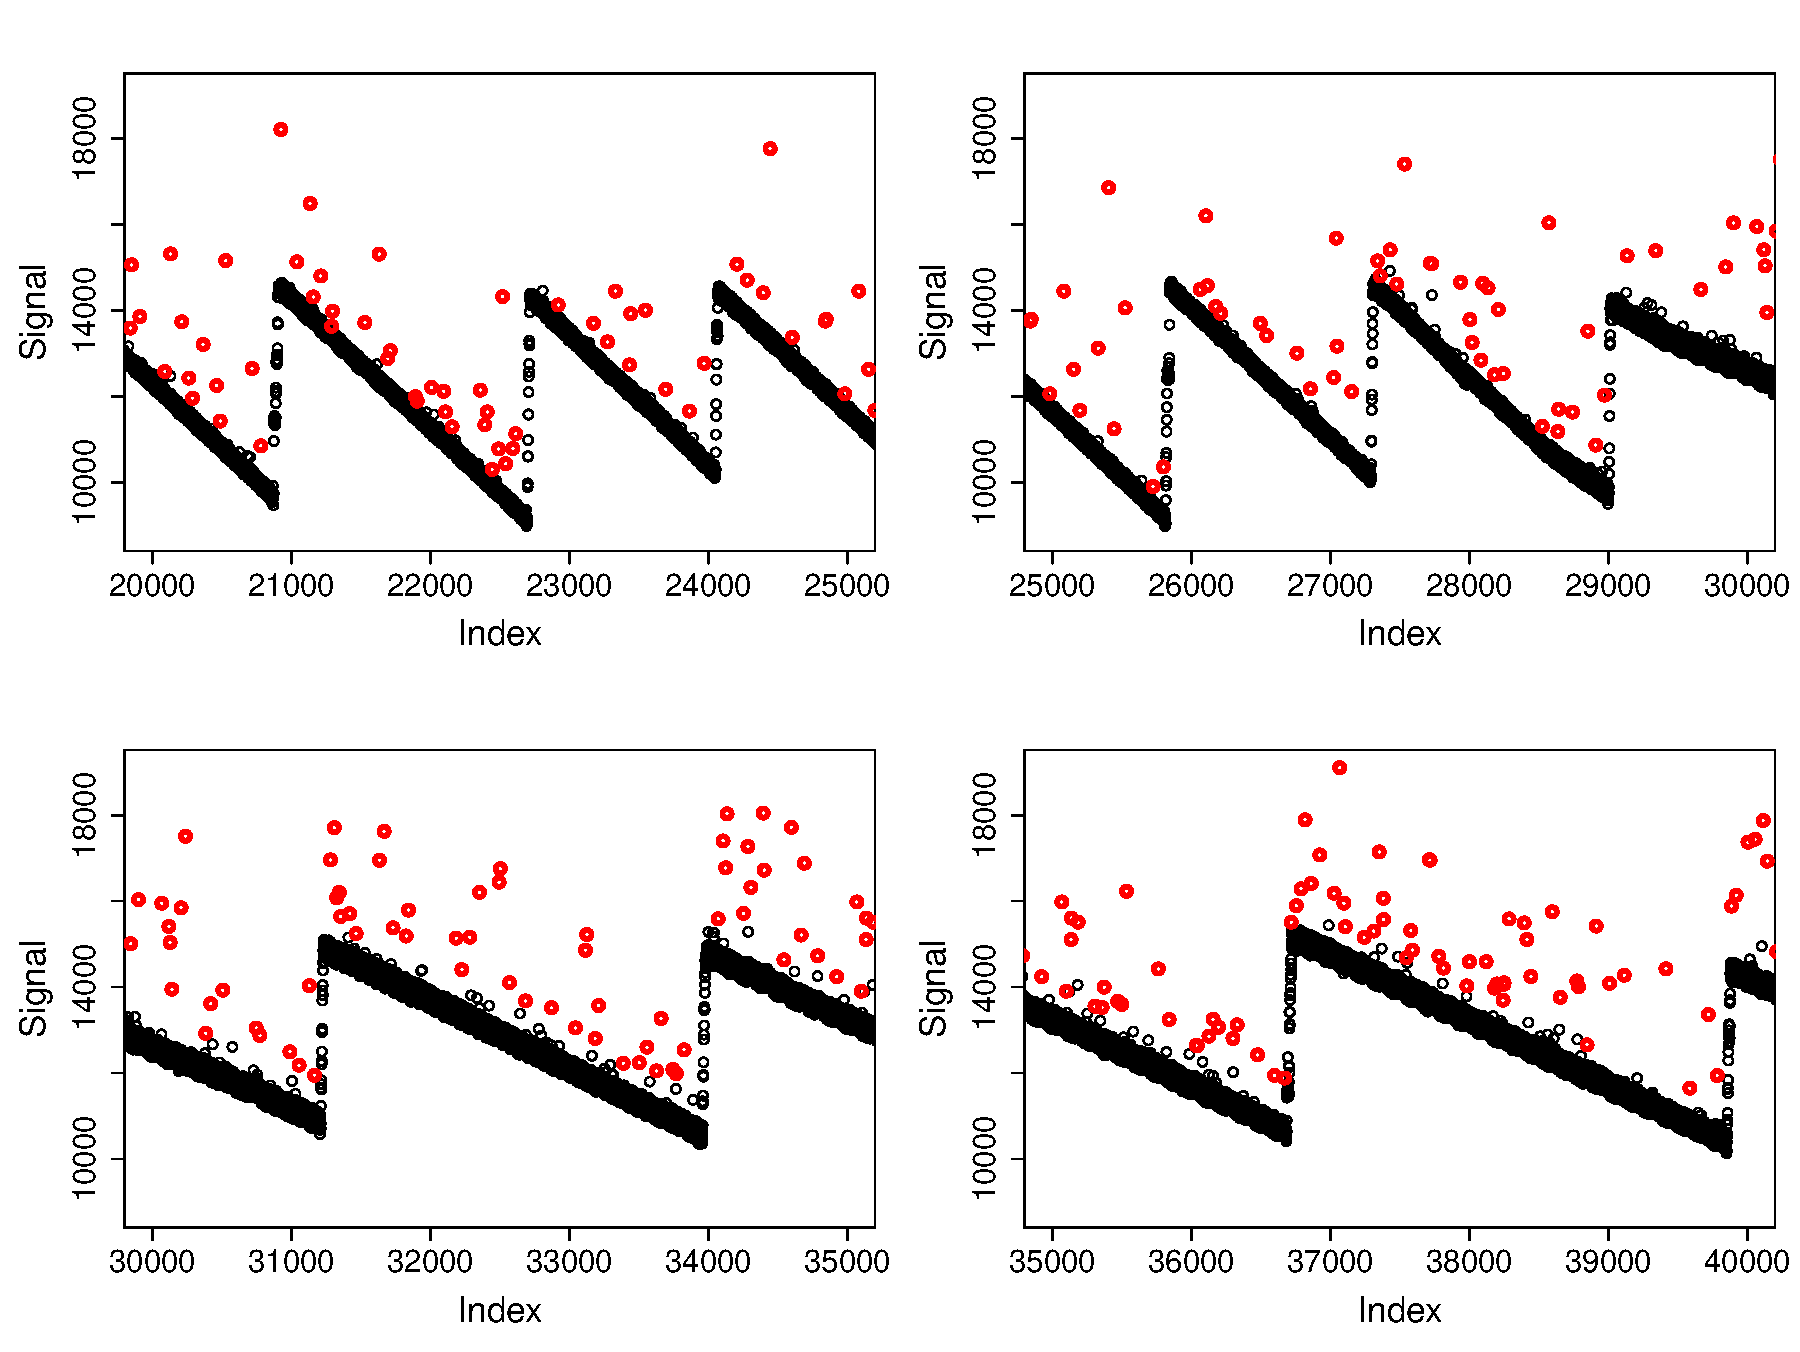
\includegraphics[width=0.45\textwidth]{pics/changeDetection/OutliersDatA4.pdf}
    \caption{Detected outliers in a CFB mass flow signal.}
    \label{fig:OutliersCFB4}
\end{figure}
Code\footnote{Code is available in GitHub repository \href{https://github.com/av-maslov/change-detection}{https://github.com/av-maslov/change-detection}}
